\chapter{Experimentación}

En este capítulo se recoge el desarrollo de los experimentos llevados a cabo en este trabajo y todos los resultados que se han obtenido empíricamente de estos.

\section{Bibliotecas y desarrollo de los experimentos}

Para el desarrollo de los experimentos usaremos las bibliotecas de aprendizaje profundo \textbf{PyTorch} para la construcción de la estructura del proyecto y \textbf{Fastai} biblioteca extensión de PyTorch para el proceso de entrenamiento de los modelos.

A continuación, podemos ver en detalle la estructura de todos nuestros experimentos.


\section{Construcción del codificador y representación latente}


\subsection{Arquitecturas con conexiones residuales: ResNet34}

\begin{table}[H]
	\centering
	\begin{tabular}{|c|c|c|c|c|}
		\hline
		epoch & train\_loss & valid\_loss & mae & time \\ \hline
		0 & 0.098790 & 0.111301 & 0.111301 & 1:09:46 \\ \hline
		1 & 0.079261 & 0.081548 & 0.081548 & 1:13:33 \\ \hline
		2 & 0.071293 & 0.075421 & 0.075421 & 1:14:20 \\ \hline
		3 & 0.064748 & 0.067580 & 0.067580 & 1:14:41 \\ \hline
		4 & 0.059911 & 0.062933 & 0.062933 & 1:15:55 \\ \hline
		5 & 0.057501 & 0.059307 & 0.059307 & 1:15:36 \\ \hline
		6 & 0.055986 & 0.058405 & 0.058405 & 1:15:37 \\ \hline
	\end{tabular}
	\caption{Pérdida de entrenamiento y validación para la reconstrucción con ResNet34}
	\label{tabla:resultados2}
\end{table}


\begin{figure}[H]
	\centering
	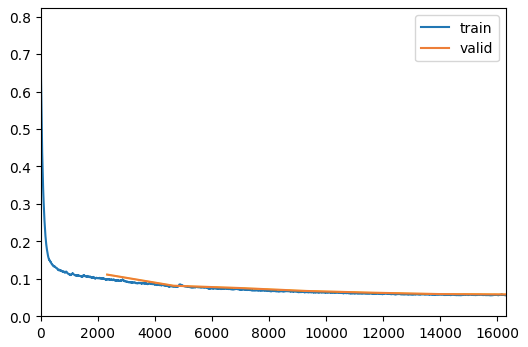
\includegraphics[width=0.8\linewidth]{imagenes/curva_resnet34.png}
	\caption{Curva de aprendizaje con ResNet34}
\end{figure}

\begin{figure}[H]
	\centering
	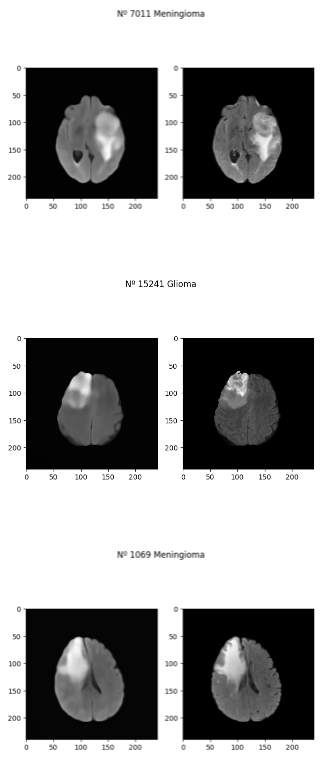
\includegraphics[width=0.5\linewidth]{imagenes/reconstruccion_resnet34.png}
	\caption{Reconstrucción de las imágenes con ResNet34}
\end{figure}

\subsection{Arquitecturas con filtros con distinto tamaño: Xception}

\begin{table}[H]
	\centering
	\begin{tabular}{|c|c|c|c|c|}
		\hline
		epoch & train\_loss & valid\_loss & MAE & time \\ \hline
		0 & 0.102650 & 0.105854 & 0.105854 & 1:24:38 \\ \hline
		1 & 0.083989 & 0.089979 & 0.089979 & 1:28:34 \\ \hline
		2 & 0.074420 & 0.085525 & 0.085525 & 1:28:33 \\ \hline
		3 & 0.068684 & 0.071334 & 0.071334 & 1:30:09 \\ \hline
		4 & 0.063998 & 0.065802 & 0.065802 & 1:26:00 \\ \hline
		5 & 0.060919 & 0.063771 & 0.063771 & 1:27:03 \\ \hline
		6 & 0.060293 & 0.062978 & 0.062978 & 1:26:51 \\ \hline
	\end{tabular}
	\caption{Pérdida de entrenamiento y validación para la reconstrucción de Xception}
	\label{tabla:resultados}
\end{table}

\begin{figure}[H]
	\centering
	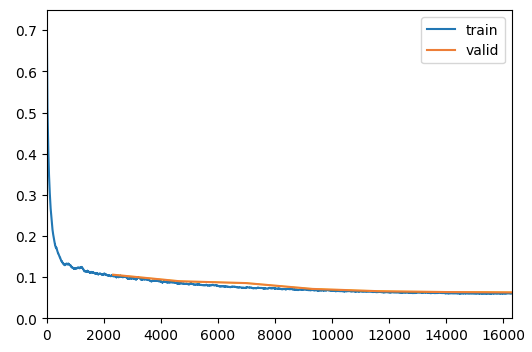
\includegraphics[width=0.8\linewidth]{imagenes/curva_xception.png}
	\caption{Curva de aprendizaje con Xception}
\end{figure}

\begin{figure}[H]
	\centering
	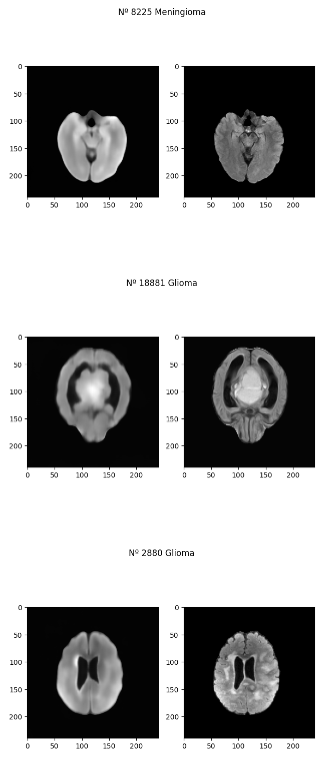
\includegraphics[width=0.5\linewidth]{imagenes/reconstruccion_xception.png}
	\caption{Reconstrucción de las imágenes con Xception}
\end{figure}

\section{Clasificación}

\begin{table}[H]
	\centering
	\begin{tabular}{|c|c|c|c|c|c|}
		\hline
		epoch & train\_loss & valid\_loss & accuracy & balanced\_accuracy & time \\ \hline
		0 & 0.112794 & 0.178968 & 0.805254 & 0.781898 & 1:04:50 \\ \hline
		1 & 0.119699 & 0.174729 & 0.819330 & 0.773066 & 1:03:01 \\ \hline
		2 & 0.083459 & 0.141255 & 0.855540 & 0.794527 & 1:04:18 \\ \hline
	\end{tabular}
	\caption{Pérdida de entrenamiento y validación para clasificación con la parte convolucional congelada}
	\label{tabla:resultados3}
\end{table}

\begin{figure}[H]
	\centering
	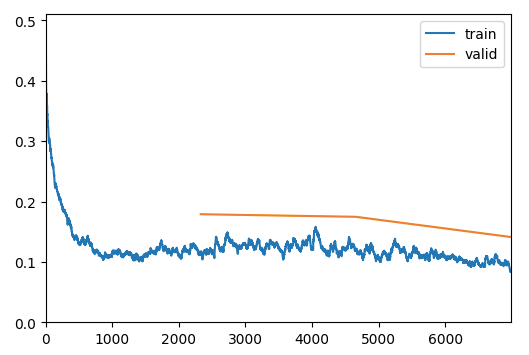
\includegraphics[width=0.8\linewidth]{imagenes/task1_freeze.png}
	\caption{Curva de aprendizaje para clasificación parte convolucional congelada}
\end{figure}

\begin{table}[H]
	\centering
	\begin{tabular}{|c|c|c|c|c|c|}
		\hline
		epoch & train\_loss & valid\_loss & accuracy & balanced\_accuracy & time \\ \hline
		0 & 0.056434 & 0.209338 & 0.855477 & 0.840139 & 1:01:57 \\ \hline
		1 & 0.040761 & 0.190361 & 0.864976 & 0.812309 & 1:01:41 \\ \hline
		2 & 0.023256 & 0.260177 & 0.876575 & 0.832247 & 1:00:26 \\ \hline
		3 & 0.009723 & 0.330192 & 0.877014 & 0.834721 & 1:00:30 \\ \hline
	\end{tabular}
	\caption{Pérdida de entrenamiento y validación para clasificación toda la red descongelada}
	\label{tabla:resultados3}
\end{table}

\begin{figure}[H]
	\centering
	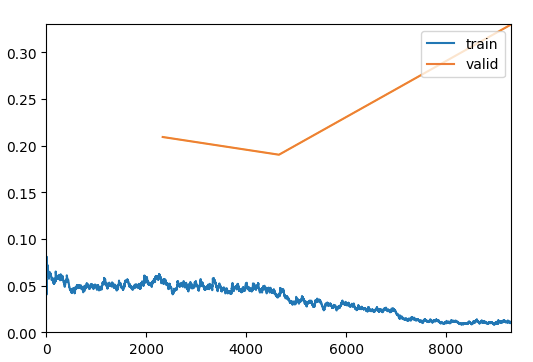
\includegraphics[width=0.8\linewidth]{imagenes/task1_unfreeze.png}
	\caption{Curva de aprendizaje para clasificación toda la red descongelada tras ajustar capas densamente conectadas}
\end{figure}

\begin{table}[H]
	\centering
	\begin{tabular}{|c|c|c|c|c|c|}
		\hline
		epoch & train\_loss & valid\_loss & accuracy & balanced\_accuracy & time \\ \hline
		0 & 0.080457 & 0.178836 & 0.854348 & 0.796523 & 1:23:49 \\ \hline
		1 & 0.084583 & 0.175143 & 0.847827 & 0.781100 & 1:24:09 \\ \hline
		2 & 0.086810 & 0.159217 & 0.852185 & 0.800501 & 1:26:20 \\ \hline
		3 & 0.081304 & 0.370888 & 0.832309 & 0.747997 & 1:21:31 \\ \hline
	\end{tabular}
	\caption{Pérdida de entrenamiento y validación para clasificación para todo el entrenamiento toda la red descongelada}
	\label{tabla:resultados6}
\end{table}


\begin{figure}[H]
	\centering
	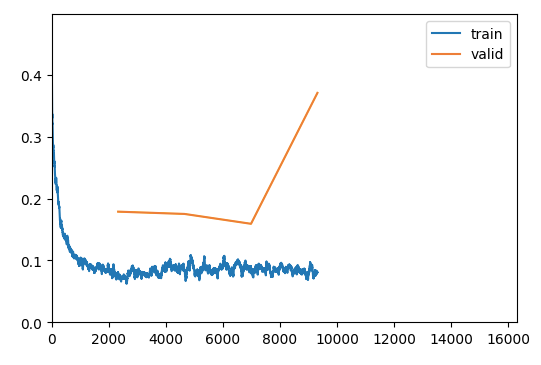
\includegraphics[width=0.8\linewidth]{imagenes/task1_totally_unfreeze.png}
	\caption{Curva de aprendizaje para clasificación todo el entrenamiento toda la red descongelada}
\end{figure}

\begin{figure}[H]
	\centering
	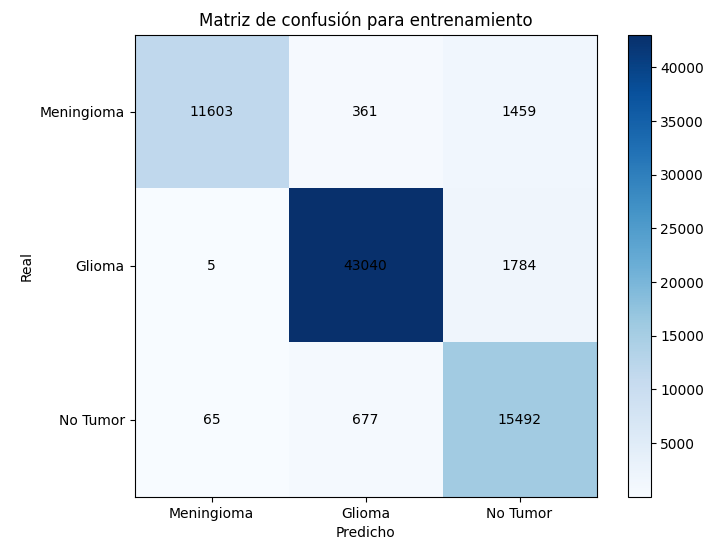
\includegraphics[width=0.8\linewidth]{imagenes/task1_results_train.png}
	\caption{Matriz de confusión de entrenamiento sin votación}
\end{figure}

\begin{figure}[H]
	\centering
	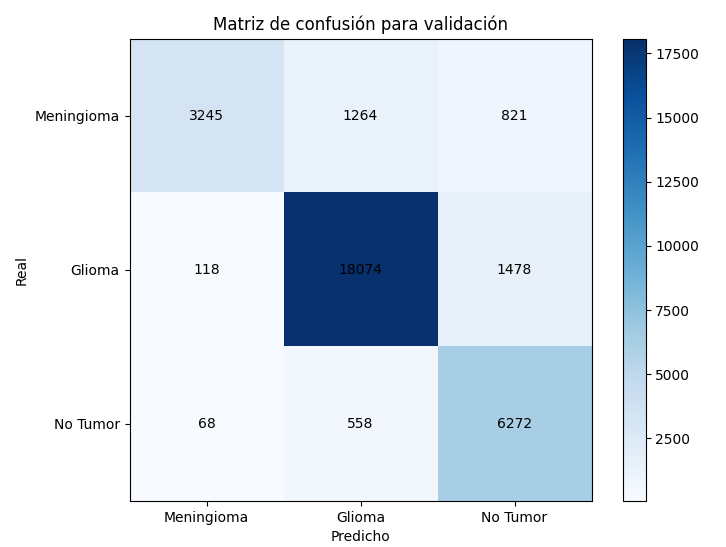
\includegraphics[width=0.8\linewidth]{imagenes/task1_results_validation.png}
	\caption{Matriz de confusión de validación sin votación}
\end{figure}

\begin{figure}[H]
	\centering
	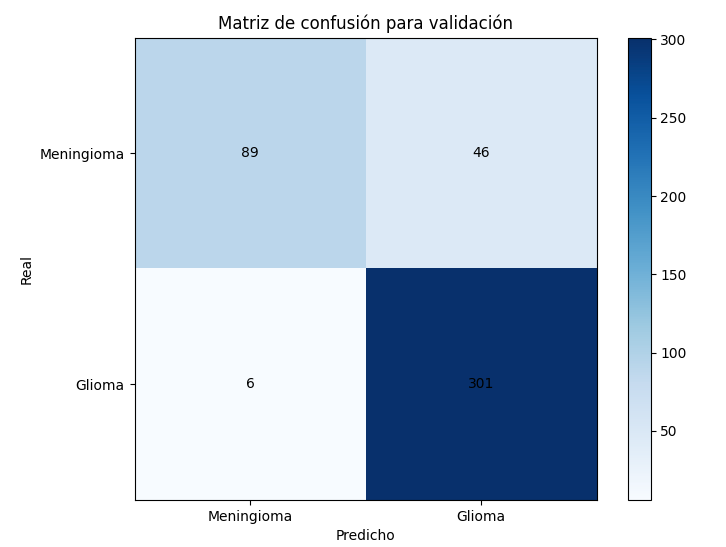
\includegraphics[width=0.8\linewidth]{imagenes/task1_val_5.png}
	\caption{Matriz de confusión de validación con votación: $Meningiomas < 5$}
\end{figure}

\begin{figure}[H]
	\centering
	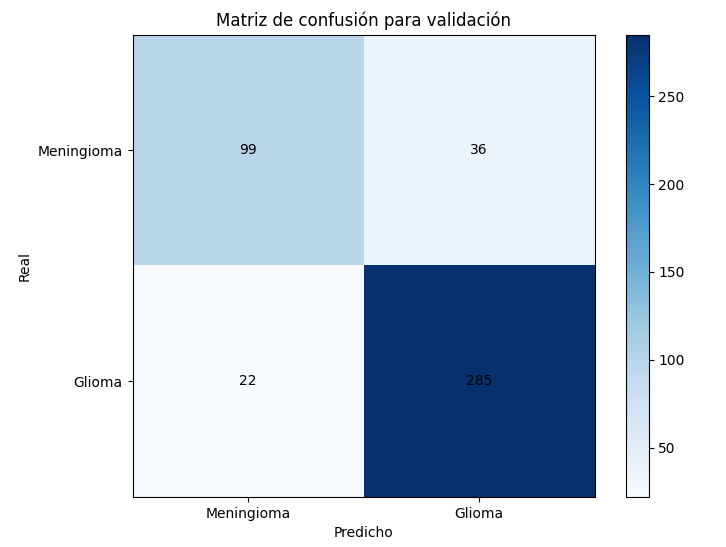
\includegraphics[width=0.8\linewidth]{imagenes/task1_val_3.png}
	\caption{Matriz de confusión de validación con votación: $Meningiomas < 3$}
\end{figure}

\begin{figure}[H]
	\centering
	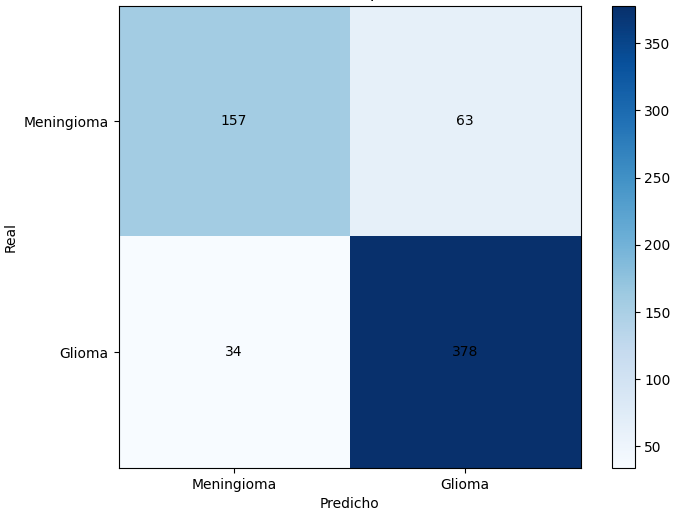
\includegraphics[width=0.8\linewidth]{imagenes/task1_test.png}
	\caption{Matriz de confusión de Test con votación}
\end{figure}


\section{Segmentación}

\begin{table}[H]
	\centering
	\begin{tabular}{|c|c|c|c|c|c|}
		\hline
		epoch & train\_loss & valid\_loss & Dice Loss & time \\ \hline
		0 & 0.095941 & 0.319656 & 0.319656 & 1:34:08 \\ \hline
		1 & 0.073242 & 0.258797 & 0.258797 & 1:32:56 \\ \hline
		2 & 0.059904 & 0.284256 & 0.284256 & 1:34:48 \\ \hline
		3 & 0.050076 & 0.274452 & 0.274452 & 1:37:00 \\ \hline
		4 & 0.046783 & 0.266702 & 0.266702 & 1:40:18 \\ \hline
	\end{tabular}
	\caption{Pérdida de entrenamiento y validación para segmentación toda la red descongelada}
	\label{tabla:resultados4}
\end{table}

\begin{figure}[H]
	\centering
	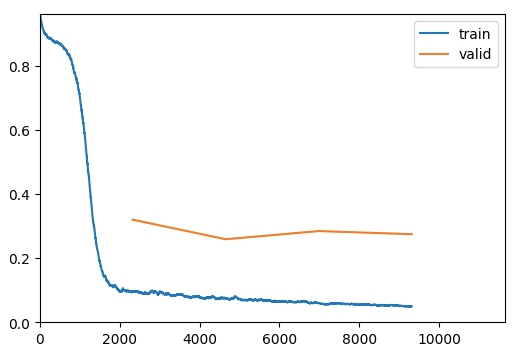
\includegraphics[width=0.8\linewidth]{imagenes/curva_segmentation.png}
	\caption{Curva de aprendizaje para la tarea de segmentación}
\end{figure}

\begin{figure}[H]
	\centering
	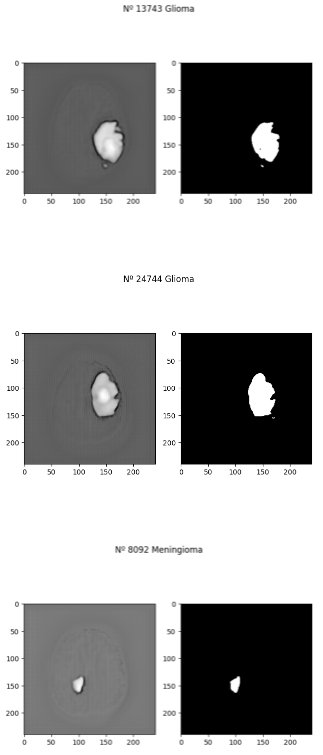
\includegraphics[width=0.5\linewidth]{imagenes/output_segmentation.png}
	\caption{Comparación de la salida del modelo respecto la real}
\end{figure}

\begin{table}[H]
	\centering
	\begin{tabular}{|c|c|c|c|}
		\hline
		Partición & Similaridad Dice & Distancia Hausdorff & Sensibilidad \\ \hline
		Validación & 0.777343 & 14.573561 & 0.720415 \\ \hline
		Test & 0.772642 & 14.577154 & 0.709075 \\ \hline
	\end{tabular}
	\caption{Resultados de hold-out en validación y test para segmentación}
	\label{tabla:resultados5}
\end{table}

\begin{figure}[H]
	\centering
	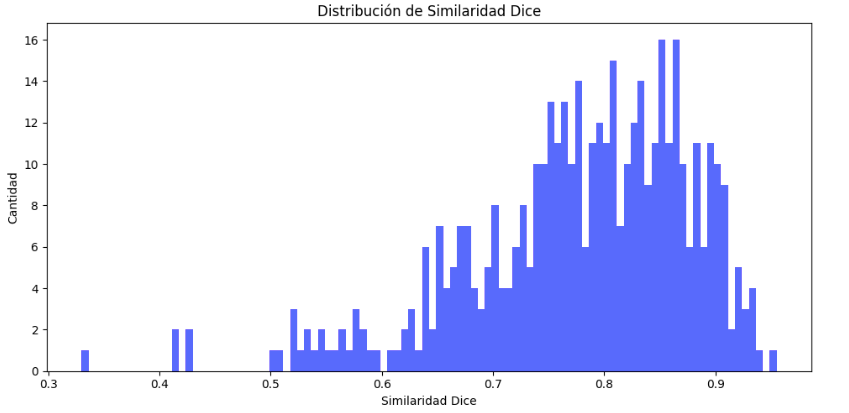
\includegraphics[width=0.75\linewidth]{imagenes/dist_dice_val.png}
	\caption{Distribución de similaridad Dice en el conjunto de validación}
\end{figure}

\begin{figure}[H]
	\centering
	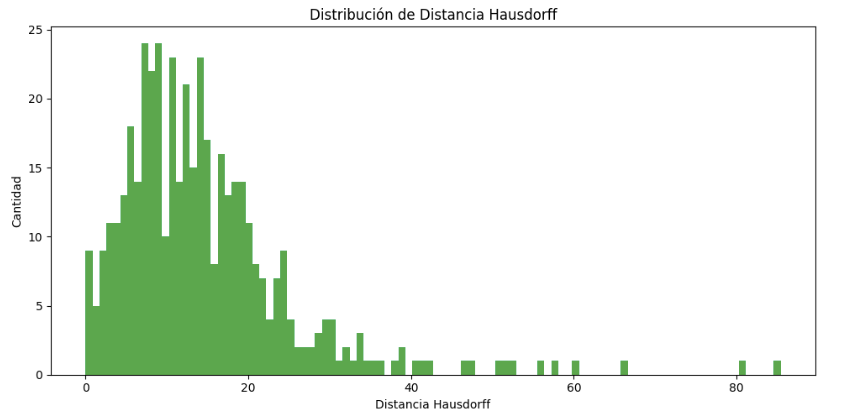
\includegraphics[width=0.75\linewidth]{imagenes/dist_haus_val.png}
	\caption{Distribución de distancia Hausdorff en el conjunto de validación}
\end{figure}

\begin{figure}[H]
	\centering
	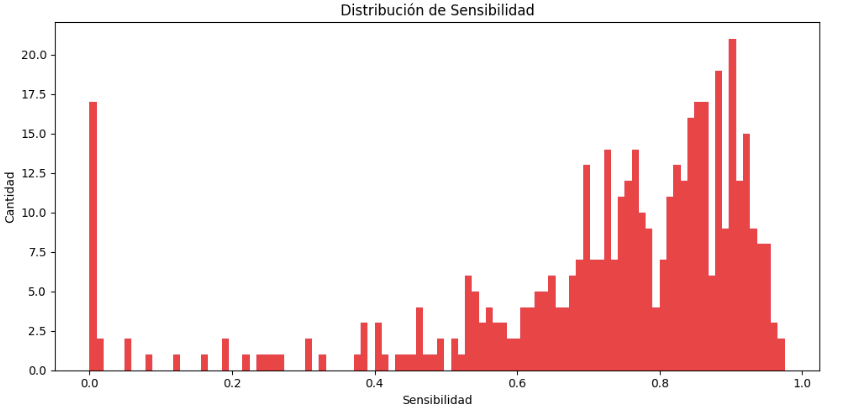
\includegraphics[width=0.75\linewidth]{imagenes/dist_sen_val.png}
	\caption{Distribución de sensibilidad en el conjunto de validación}
\end{figure}

\begin{figure}[H]
	\centering
	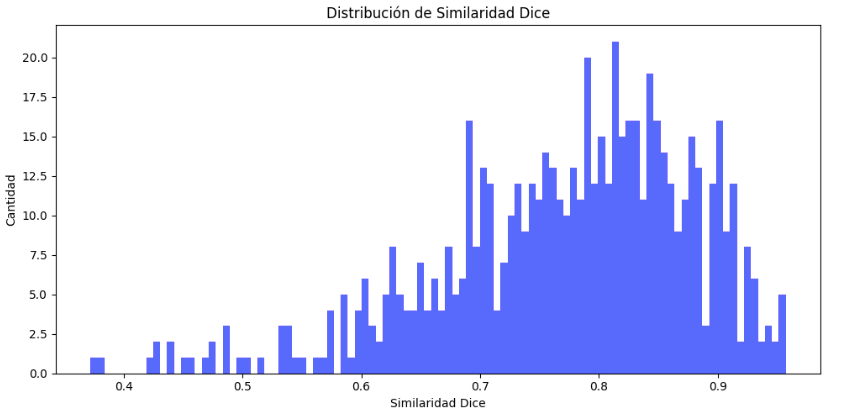
\includegraphics[width=0.75\linewidth]{imagenes/dist_dice_test.png}
	\caption{Distribución de similaridad Dice en el conjunto de test}
\end{figure}

\begin{figure}[H]
	\centering
	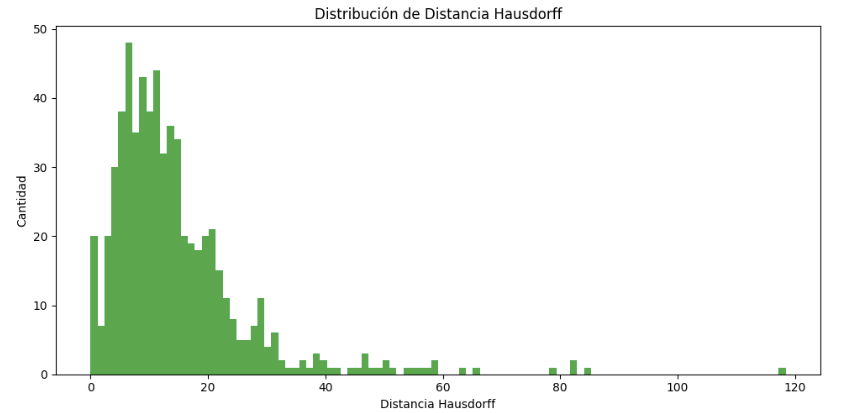
\includegraphics[width=0.75\linewidth]{imagenes/dist_haus_test.png}
	\caption{Distribución de distancia Hausdorff en el conjunto de test}
\end{figure}

\begin{figure}[H]
	\centering
	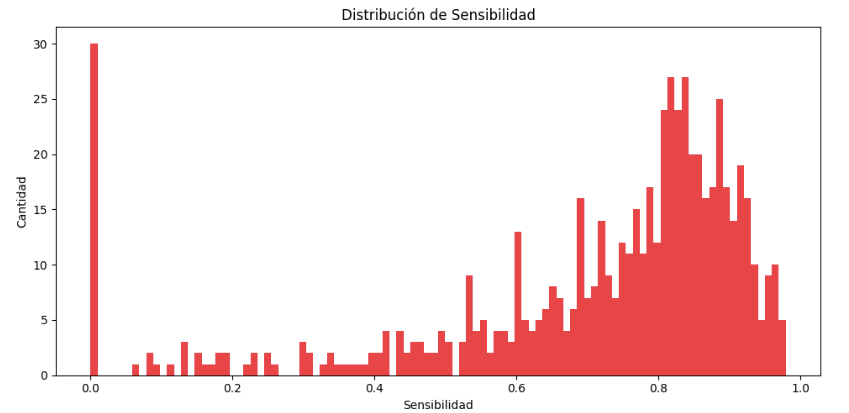
\includegraphics[width=0.75\linewidth]{imagenes/dist_sen_test.png}
	\caption{Distribución de sensibilidad en el conjunto de test}
\end{figure}